\section{Artificial Neural Networks}
To understand neural networks, first it is necessary to understand it's building blocks, artificial neurons. Commonly called just neurons, nodes, or units (the preferred term used in this document will be unit), these were historically inspired by biological neurons. The idea behind them is that a single unit is a very simple element that receives some inputs and produces an output, the real power comes from connecting many of these together, from thousands, to millions, or even billions of connections\footnote{
  As of writing this document GPT-3 is the biggest neural network model of all time, having 175 billion parameters \cite{gpt3_2020}.
}.
\begin{figure}[hbt]
    \centering
    \caption{Single unit representation}
    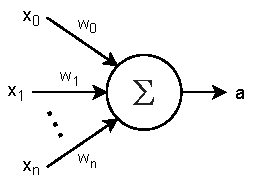
\includegraphics[width=0.4\textwidth]{chapters/NeuralNets/figures/neuron.pdf}
    \fonte{From the author (2021)}
    \label{fig:neuron}
\end{figure}

\autoref{fig:neuron} shows a representation of an artificial unit, it receives a set of inputs $[x_0, x_1, ..., x_n]$, denoted as a vector $\bm{x}$, and each input has a corresponding scalar value $w_i$ called it's weight. Units will also often have a bias term $b$ that is independent of the inputs and that is useful for shifting the output.

By changing the set of weights (in vector form $\bm{w}$) and the bias term, it is possible to achieve different behaviours from the unit based on it's inputs. \autoref{eq:weighted_input} shows how these parameters are used to calculate what is called the \textit{weighted input} ($z$) of the unit \cite[Chapter 2]{NN&DL2015}.
\begin{equation} \label{eq:weighted_input}
    z = \sum_{i}^{n}{w_i x_i} + b =
    %
    \begin{bmatrix}w_0, & w_1, & ... & w_n\end{bmatrix}^T
    \begin{bmatrix}x_0, & x_1, & ... & x_n\end{bmatrix} + b =
    %
    \bm{w}^T \cdot \bm{x} + b
\end{equation}

The weighted input is usually passed through a non-linear function $f$, called the \textit{activation function}, to produce the output $a$, called the unit activation, as seen in \autoref{eq:activation}.
\begin{equation} \label{eq:activation}
    a = f\left(z\right) = f\left(\bm{w}^T \cdot \bm{x} + b\right)
\end{equation}

A neural network is built by combining multiple units together and the learning process consists of adjusting all the weights and biases in order to produce the expected results given the dataset. Any combination of connections can be considered a neural network, however for the overwhelming majority of cases the networks are divided into layers, and for most of these cases the connections form an acyclic graph. This means that there are no cycles in the network, the input flows from one layer to the next, and there is usually no connection between layers that are not consecutive \textbf{--} exceptions to this are \gls{LSTM} networks \cite{lstm1997} and Residual Networks \cite{resnet2015}, but they are not the focus of this document.

The layers of the network are commonly divided into input layer, hidden layers, and output layer. The input layer represents the input data, usually in diagram representations the inputs are drawn like units, this however is just an stylistic choice since the values do not pass through any calculation in this layer.

The output layer contains the units that will be interpreted as the result produced from the input. For example, in a case where the network is trying to predict the price of apartments given area, number of rooms, and others properties (classical machine learning example), the output would be a single unit whose activation is the predicted price. Problems where the output can assume a range of values are usually called \textit{regression} problems.

On the other hand, problems where the output is better interpreted as a discrete value are called \textit{classification} problems. Predicting the digits of \gls{MNIST} falls into the category of classification problems, where the output represents which of the 10 possible digits the input image represents.

In the case of \gls{MNIST} the output layer can be made of 10 units, where each of the activations gives the probability of the input belonging to the corresponding digit. A natural question to raise from this description is: why would there be a need for one unit to represent each class, when the number 10 can be more efficiently represented using only 4 bits (4 units)? Or even, why not use just one unit that outputs the predicted number?

One reason for this is that these simpler representations would lose the property of interpretability of the output as a probability distribution. But the most important reason can be validated empirically, it is easier for a network to classify the inputs into isolated units then it is to try and correlate them with specific bits for each class \cite[Chapter 1]{NN&DL2015} or to reduce the output into a single unit.

For most classification problems using a neural network the output layer will contain one unit for each possible class and the desired output will be a vector where all elements are 0's, except for the element corresponding to the true label that will be a 1, indicating the 100\% probability for that class. This way of encoding the outputs is called \textit{one-hot encoding}.


The rest of the layers in a neural network, called the hidden layers, are all the layers between the input and output. A neural network does not need to have any hidden layers, but they are fundamental for building more complex relations and robust models.

\textcite{universalApproximator1989} showed that, given sufficient hidden units, any neural network with a single hidden layer can be used to approximate any function to any amount of precision, in other words, neural networks with at least a hidden layer are \textit{universal approximators}. But in practice it is observed that more hidden layers usually perform better, they are able to divide the problems into steps and gradually reach the result. For example, an image classifier might use the first layers to distinguish lower level features like edges, while deeper layers recognize shapes, textures, and all the way to complex patterns like faces \cite{deepLearningBook2016}.

More recent years have seen a resurgence of \gls{DL}, this is generally understood as learning with networks having at least two hidden layers, but modern models can have much more than that\footnote{
    Google's Inception v3 image classifier model has 42 layers in total \cite{inceptionV3_2015}
}.

\autoref{fig:network} shows an example of the layered structure of a neural network, for simplicity the diagram shows only fully connected layers (all the units of a layer are connected to all the units of the previous layer, see \autoref{subsub:fully_connected}) but it could also have different types of layer without losing the general idea of input, hidden, and output.
\begin{figure}[hbt]
    \centering
    \caption{Diagram of a fully connected neural network}
    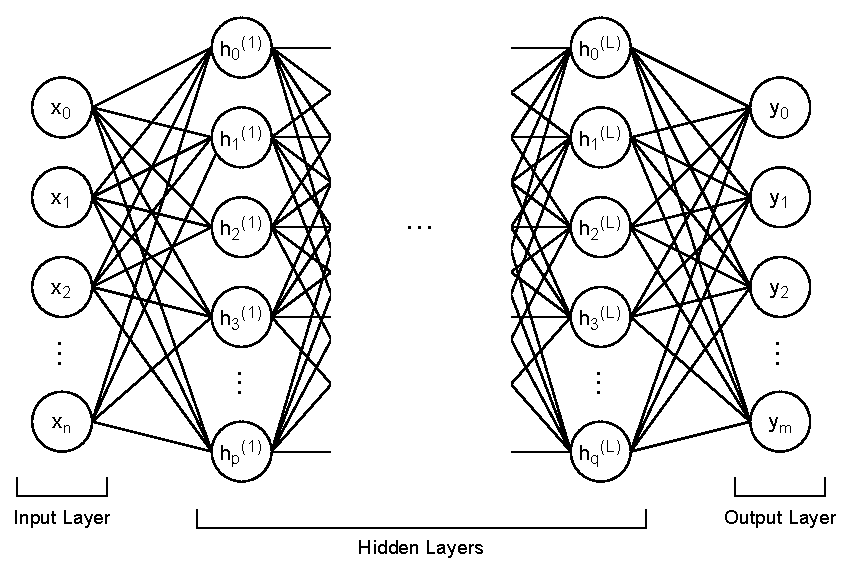
\includegraphics[width=0.8\textwidth]{chapters/NeuralNets/figures/network.pdf}
    \fonte{From the author (2021)}
    \label{fig:network}
\end{figure}


\subsection{Types of layers}
The networks constructed for this document will all use a combination of fully connected and convolutional layers. This section will explain how these work, how they differ, and their advantages in relation to each other.

Before proceeding however, it is important to define the notation that will be used. Since from now on the focus will changes from single units to an entire network, it is necessary to establish a notation that allows for indexing individual units, in any layer, and also their parameters.

The bias, weighted input, and activation for unit $i$ in layer $l$ will be written as $b_{i}^{(l)}$, $z_{i}^{(l)}$, and $a_{i}^{(l)}$ respectively. The weight connecting unit $j$ in layer $l-1$, to unit $i$ in layer $l$ will be written as $w_{ij}^{(l)}$.

The set of biases, weighted inputs, and activations in layer $l$ can also be written as the vectors $\bm{b}^{(l)}$, $\bm{z}^{(l)}$ and $\bm{a}^{(l)}$. The weights connecting the units in layer $l-1$ to units in layer $l$ can be written as the weight matrix $\bm{W}^{(l)}$.
\begin{equation*}
    \renewcommand{\arraystretch}{1.4}
    \setlength\arraycolsep{4pt}
    \bm{z}^{(l)} = \begin{bmatrix}
        z_{0}^{(l)} \\
        z_{1}^{(l)} \\
        \vdots \\
        z_{n}^{(l)}
    \end{bmatrix}
    %
    \quad
    \bm{a}^{(l)} = \begin{bmatrix}
        a_{0}^{(l)} \\
        a_{1}^{(l)} \\
        \vdots \\
        a_{n}^{(l)}
    \end{bmatrix}
    %
    \quad
    \bm{b}^{(l)} = \begin{bmatrix}
        b_{0}^{(l)} \\
        b_{1}^{(l)} \\
        \vdots \\
        b_{n}^{(l)}
    \end{bmatrix}
    %
    \quad
    \bm{W}^{(l)} = \begin{bmatrix}
        w_{00}^{(l)} & w_{01}^{(l)} & \dots  & w_{0m}^{(l)} \\
        w_{10}^{(l)} & w_{11}^{(l)} & \dots  & w_{1m}^{(l)} \\
        \vdots       & \vdots       & \ddots & \vdots \\
        w_{n0}^{(l)} & w_{n1}^{(l)} & \dots  & w_{nm}^{(l)}
    \end{bmatrix}
\end{equation*}

Recall that the activation of a unit is simply it's activation function, denoted here as $f$, applied to the weighted input. \autoref{eq:activation_again} rewrites this relation as shown in \autoref{eq:activation} using the revised notation.
\begin{equation} \label{eq:activation_again}
    \bm{a}^{(l)} = f\left( \bm{z}^{(l)} \right)
\end{equation}

Observe that in \autoref{eq:activation_again} the activation function is applied to the vector $\bm{z}^{(l)}$, this is a common shorthand notation to represent the element-wise application of the function to the vector. This notation will be used throughout the entirety of this document, all functions applied to vectors will be applied element-wise unless otherwise noted.

\subsubsection{Fully connected layer} \label{subsub:fully_connected}
Fully connected, also called Dense layers, are a type of layer where all the inputs are connected to all outputs of the previous layer. \autoref{eq:dense_weighted_input} shows how the weighted inputs of this layer are calculated from the activations of the previous layer.
\begin{equation} \label{eq:dense_weighted_input}
    z_{i}^{(l)} = \sum_{j}{w_{ij}^{(l)} a_{j}^{(l-1)}} + b_i^{(l)}
\end{equation}

If the previous layer is the input layer, the values for $\bm{a}^{(l-1)}$ will be the input of the network. To abstract the type of input it is useful to just replace the notation with a general layer input $\bm{x}$. The activation can be written more simply by using vector form as shown in \autoref{eq:dense_activation}, the layer superscripts were also omitted for more clarity.
\begin{equation} \label{eq:dense_activation}
    \bm{a} = f\left( \bm{W}\bm{x} + \bm{b} \right)
\end{equation}

Dense layers are extremely common, being used in many types of neural networks. They are very useful for mapping their inputs, that can have any number of dimensions, to a vector with any different number of dimensions, this is used in almost all classifiers to reduce the detected features into a one-hot encoded vector of the possible classes. For example, in the 2012 ImageNet challenge the three last layers of the network AlexNet were fully connected, they mapped the $43,264$ features into a $1000$ dimensional vector corresponding to all classes of images in the challenge \cite{alexnet2012}.

This type of layer can also be used to apply transformations to features that will be used later in the network, this is used in \acp{GAN} to map the latent space to a vector that is transformed into the generated image (see\autoref{cha:gans}). They can even be used for full feature extraction, but this is usually not the best choice since they are quite expensive given the high number of connections and, as will be seen, they lack some useful properties that are present in convolutional layers.


\subsubsection{Convolutional layer}
One drawback of fully connected layers is that they do not leverage the structure of the data when calculating the activations. Consider for example the case of images, when dealing with random values all pixels are uncorrelated with one another, but in real world situations the pixels of an image group together to make edges, shapes and complex figures. The same could be said for audio, video, language and many other situations \cite{guide_conv2018}.

Consider the example of a simple image of a digit in the \gls{MNIST} dataset, by translating the image by a couple of pixels or by slightly warping the strokes the digit represented does not change. But since the fully connected layer has no sense of neighbouring pixels (or temporal coherence for audio and video, etc.), then it has no choice other than learning weights for all possible slight transformations to the inputs. This not only makes learning more difficult, but also introduces many unnecessary parameters to the network.

Convolutional layers are a way of dealing with this problem. Initially inspired by the visual cortex of vertebrates \cite{neurocognitron1982}, the idea behind them is to detect the presence of features, no matter where they are present or if they are slight perturbed (e.g. an edge should be seen as an edge, no matter where it is located in the image or if it is slightly rotated).

Neural networks that employ convolutional layers are usually called \acp{CNN}, their history is very long and they were already used in the 1990's for learning the \gls{MNIST} dataset when it was introduced \cite{mnist1998}. However they were not very popular for larger problems and only grew in popularity after the great breakthrough in the ImageNet challenge achieved by the \gls{CNN} AlexNet in 2012 \cite{alexnet2012}. Since then they have become very common and are used in a variety of situations, even outside of image recognition. 

This section will only explain how they work for the 2-dimensional case, but the idea can be easily generalized to the 1-dimensional or multidimensional cases. The inputs of a convolutional layer share the properties that they are represented as multidimensional arrays, have one or more axis where the ordering matters (for images these are the width and height), and can have an axis representing different views of the data (e.g. the RGB channels for a colored image) \cite{guide_conv2018}.

The name convolution is not a coincidence, the layer operation is related to the convolutions seen in signal processing for 1D discrete signals, the image convolutions like gaussian and Sobel filters, or higher dimensions mathematical convolutions. The operation consists of sliding a window of weights, called the kernel, over the entire input and calculating the sum of the weighted inputs covered by this window to produce the resulting values.
\begin{figure}[hbt]
    \centering
    \caption{Convolutional layer kernel properties}
    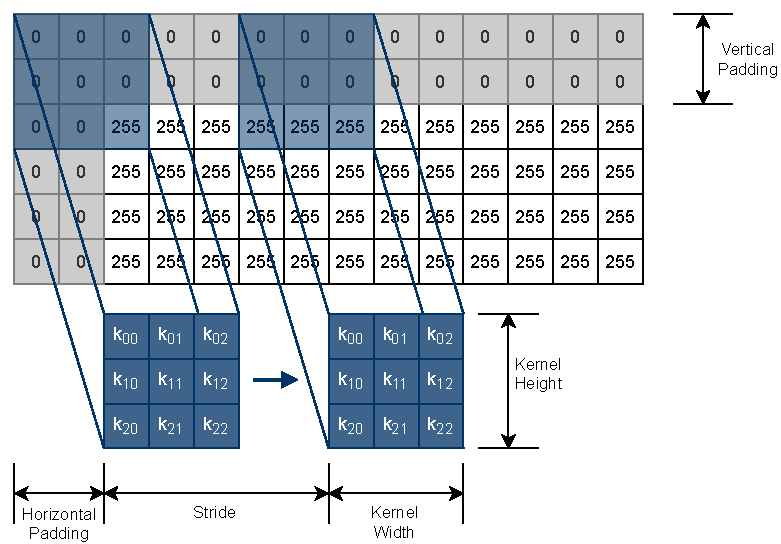
\includegraphics[width=0.55\textwidth]{chapters/NeuralNets/figures/cnn.pdf}
    \fonte{From the author (2021)}
    \label{fig:kernel_properties}
\end{figure}

It is simpler to understand this by looking at an image representation, \autoref{fig:kernel_properties} shows an example of a kernel being applied at the corner of an image with a single channel, whose values are $255$, and that is padded with zeros.

As seen in the figure, the kernel will start at the top left of the image (including some optional zero padding) and calculate a value for that position, then it will step a number of pixels, called the stride, and calculate the next value. When there is no more room to step horizontally, the kernel will start again at the left of the image and step a stride size downward, this is repeated until the whole image is traversed.

The convolution value between the kernel window and the pixels is simply the sum of the element wise products between the pixel values and the corresponding kernel weight. An image can be used again to help visualize this process, \autoref{fig:convolution} shows how a convolution is calculated for a $3\times3$ kernel, on a $3\times3$ image, with $1$ pixel zero padding, and stride of $1$ for both horizontal and vertical directions.
\begin{figure}[hbt]
    \centering
    \caption{Simple convolution process}
    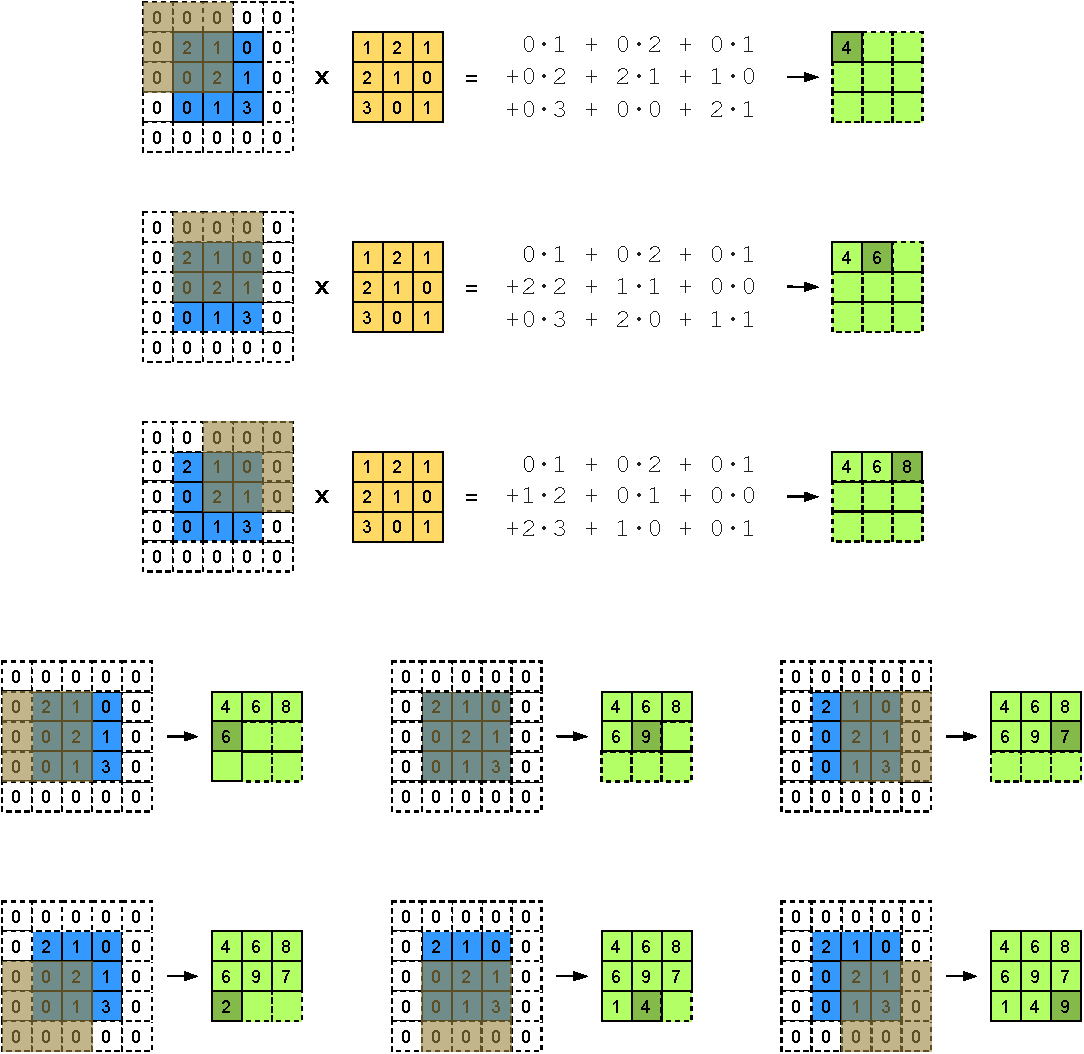
\includegraphics[width=0.7\textwidth]{chapters/NeuralNets/figures/convolution.pdf}
    \fonte{From the author (2021)}
    \label{fig:convolution}
\end{figure}

Also note that the kernel does not change when calculating the outputs of the convolution, in other words, the weights of the kernel are shared between the units. These weight are learned instead of being predefined, this allows for the network to decide which features the kernels should detect in order to solve the problem; these could be for example edges, textures, shapes, specific colors or others.

One important detail to mention is that the examples shown until now only consist of single channel images. For colored images with 3 channels, and more general cases with $n$ channels, the kernel is not just a 2D matrix but is more accurately represented as a volume (i.e. one 2D kernel for each channel) . This means that in \autoref{fig:convolution} the kernel is a $3\times3\times1$ volume, if the input were a colored image it would be a $3\times3\times3$ volume. For the general case of an $n$ channel input, the volume would be $h\times w\times n$ for a kernel with height $h$ and width $w$.

The convolution for multiple channels is basically the same as for a single channel, each $h\times w$ slice of the volume is convoluted with one of the channels and the results are added together to get the final convolution. These resulting values can be considered as the weighted inputs $\bm{z}$ of the convolutional layer, so the activation function should be applied in order to get the final layer output.

In summary, for the case of images, a convolutional layer takes as input a 3D volume (i.e. two spatial dimensions to convolve with, and 1 channel dimension to give different views of the image) and operates on it using a kernel volume, the spatial sizes of the kernel are free to choose, but the number of channels must match. The convolution operation with a single kernel will reduce the input volume to a 2D feature map, where each point in the map indicates how much the feature is present at that region of the input covered by the kernel window. In general it is desirable to detect many different features from the input image, this means that convolutional layers will have multiple kernels and all the resulting convolutions will be stacked to produce an output volume.

The output will have as many channels as the number of kernels used in the convolutional layer, but the width and height will depend on the kernel size, stride, and padding. Consider sliding the kernel in the horizontal direction (the same logic applies to any direction and for all input dimensions), the number of values calculated by the convolution will be the number of possible positions that the kernel can be placed in this direction.

Suppose that in the horizontal direction the sizes of input, kernel, zero padding, and stride are $i$, $k$, $p$, and $s$ respectively. Then the output size $o$ in this direction is given by \autoref{eq:conv_output_size} \cite{guide_conv2018}, where $\lfloor{.}\rfloor$ is the floor function.
\begin{equation} \label{eq:conv_output_size}
    o = \left\lfloor{
        \frac{i + 2p - k}{s}
    }\right\rfloor + 1
\end{equation}

Convolutions can be used to enlarge the input image, but are most commonly used to reduce the dimensions while raising the number of features detected. For example, the GoogLeNet Inception architecture reduces the $224\times224\times3$ input image to a feature map of size $7\times7\times1024$ \cite{inceptionV1_2014}. This reduction is usually not done using only a single convolutional layer, it is most common for the input volume to pass through multiple convolutions that gradually reduce it's width and height while increasing it's depth. Looking at the Inception model again, the whole network is $22$ layers deep with most of those being convolutions for feature extraction \cite{inceptionV1_2014}.

According to \textcite[chap. 9]{deepLearningBook2016}, convolutional layers leverage the ideas of sparse interactions, shared parameters, and equivariant representations to improve a machine learning system. They describe sparse interactions in the sense that kernels are smaller than the input, reducing the number of parameters, the memory used, the processing cost, and improving statistical efficiency. And the idea of equivariant representations is related with the invariance to translation, since at least in principle, the use of a sliding window allows for detecting the same feature no matter where it might appear on the image.

\subsubsection{Transposed Convolutions}
Any convolution operation can be converted to a matrix multiplication where the input is flattened to a 1-dimensional vector and the kernel is converted to a sparse matrix $\bm{C}$. The forward pass through the network, which is when the convolution is applied, is equivalent to multiplying the flattened input by $\bm{C}$, and the backward pass is equivalent with multiplying by $\bm{C}^T$ \cite{guide_conv2018}. The multiplication with $\bm{C}^T$ converts the output volume to the input volume and is commonly called the transposed convolution, or sometimes \textit{deconvolution}.

Any kernel represents both a convolution or transposed convolution, it all depends on how the values are interpreted as a matrix. It is important to note that the transposed convolution is not a way to reverse the convolution step, it is generally not possible to calculate the input of a convolution based on the kernel and output values. But the transpose operation can be considered as a reverse in the sense of transforming the output volume into the input volume.

Given the property of producing the opposite volume in relation to convolutions, transposed convolution layers are commonly used to upscale data to higher dimensions. For example, they are used in \acp{GAN} to upscale the latent space vector into the corresponding image (see\autoref{cha:gans}) \cite{nipsGAN2017}. However, upscaling with this method has been shown to produce image artifacts \cite{deconvolutionArtifacts2016} and some models, like styleGAN \cite{styleGAN2018}, already drop the use of transposed convolution layers for different upscaling approaches.

\subsubsection{Pooling layer}
Pooling layers are very similar to convolutional layers in the sense that they both slide an window of some width and height through the image, using some stride value, optional padding, and producing a number for each possible position of the window. But pooling layers do not have any learnable parameters and just execute a predefined function over all the inputs inside the sliding window to produce the output.

The two most common types of pooling are max and average pooling. Max pooling, as the name suggests, simply returns the maximum value present in the sliding window, while average pooling returns the average of those values. Pooling layers are very commonly used together with convolutional layers, \textcite[p. 355-336]{deepLearningBook2016} describe that a usual convolutional layer in a \gls{CNN} consists of a convolution operation, followed by the nonlinear activation, and lastly by a pooling layer; they say that this operation helps to make the representation approximately invariant to input translations.

\subsubsection{Embedding Layer}
This layer is an alternative way of representing discrete valued inputs. Recall that one way to represent a discrete value (e.g. the class of a given input) is to use one-hot encoding, this allows for mapping $n$ possible values into a $n$ dimensional vector of all 0's and a single 1 representing the value.

Embedding layers offer a way to map $n$ values into a vector with $m$ dimensions, where $m$ can be any number. The mapping from value to vector in an embedding layer is not something fixed, but is also learned during training. This type of layer is very useful in language models, where encoding thousands of possible words into one-hot vectors is infeasible, embeddings allow for much smaller representations that can be learned by the model to best fit a given problem.

When conditioning \acp{GAN} with class information for the \glsunset{CGAN} \gls{CGAN} variant (see \autoref{sub:cgan}), it is necessary to combine the label of the data together with the input. Embedding layers offer a more robust solution to this when compared to one-hot vectors, because of that they were used for conditioning in the experiments seen in\autoref{cha:experiments}.


\subsection{Activation Functions}
Historically one of the first implementations of artificial neural networks used the step function as activation for the units \cite[Chapter 1]{NN&DL2015}, this means that for positive inputs the step function produces a $1$ and for all other values it produces a $0$. It also could use the sign function \cite{thePerceptron2017}, producing a $-1$ for non positive inputs.

This type of approach is called a Perceptron, one notable example of it's implementation was the MARK I Perceptron, a hardware solution where all weights were regulated by potentiometers and automatically adjusted by motors to train the network \cite{perceptron1960}. However it was later shown that this type of binary activation was very limited and could only solve linear separable problems \cite{thePerceptron2017}.

One may question the need for activation functions or why do they need to be nonlinear, what is the reason for introducing nonlinearity to the network? To understand this, first note that not using an activation function is the same as setting the output $y = x$, this is also a linear relationship between the values, so it is only necessary to explain why a linear activation is a problem.

The nonlinearity is introduced to make the network able to learn more complex relationships in the data, since not all real world situations have a linear dependence between input and output. By transforming the input through multiple nonlinear activations it is possible to create very elaborate mappings from input to output. This does not hold true for linear transformations, since applying a sequence of them to some input is equivalent to applying just a single one.

To see this consider an input vector $\bm{x}$ with two transformations matrices $\bm{A}_1$, $\bm{A}_2$ and vectors $\bm{b}_1$, $\bm{b}_2$. The output $\bm{y}_2$ is obtained by applying two linear transformations to the input vector as follows.
\begin{equation} \label{eq:linearity_1}
    \bm{y}_1 = \bm{A}_1 \bm{x} + \bm{b}_1
    \qquad \text{and} \qquad
    \bm{y}_2 = \bm{A}_2 \bm{y}_1 + \bm{b}_2 \\
\end{equation}

By rearranging the terms it can be confirmed that the two linear transformations are equivalent to a single one, this can be seen by the following derivation.
\begin{align*}
    \bm{y}_2& = \bm{A}_2 (\bm{A}_1 \bm{x} + \bm{b}_1) + \bm{b}_2 \\
    & = \bm{A}_2 \bm{A}_1 \bm{x} +  \bm{A}_2 \bm{b}_1 + \bm{b}_2 \\
    & = \bm{A} \bm{x} + \bm{b}
\end{align*}

This logic holds true for any number of linear transformations. Now it should be hopefully clear to see that there is inherently no difference between a multilayered neural network with linear activations and a simple two layered input-output network. It is necessary to introduce nonlinearities in the hidden layers in order to build more complex models \textbf{--} linear transformations can however be used in the output layer to map the values to a more desirable range, regression problems are an example.

Although nonlinear, the binary property of the step function limits the capabilities of a neural network, to work around this limitations it is necessary to introduce a different type of activation. To avoid the problem of jumping values it is best to have a continuous function instead of a discrete one, it is also important that this function be differentiable in it's domain and that the derivatives are not zero everywhere (see \glsunset{ReLU} \gls{ReLU} activation in \autoref{subsub:relu} for more remarks about this restrictions). The derivative requirements are necessary to make possible the use of the learning algorithm Gradient Descent with Backpropagation (see sections \ref{sec:loss_&_gradient_descent} and \ref{sec:backpropagation}).

This section will briefly introduce some important activation functions that are widely used in multiple machine learning problems and that were used in the experiments found in\autoref{cha:experiments}.

\subsubsection{Sigmoid} \label{subsub:sigmoid}
Usually denoted by \gls{sigmoid}, the sigmoid function maps all real numbers to the interval $(0, 1)$. For a given input $x$, the value for $\sigma(x)$ is given by \autoref{eq:sigmoid}.
\begin{equation} \label{eq:sigmoid}
    \gls{sigmoid}(x) = \frac{1}{1 + e ^ {-x}}
\end{equation}

The sigmoid function can be considered the continuous version of the step function, as the absolute value of $x$ grows, $\sigma(x)$ gets exponentially closer to $\mathsf{step}(x)$, but there is a continuous transition close to $0$. This can be seen more clearly in\autoref{fig:activations}.
\begin{figure}[hbt]
    \centering
    \caption{Curves of sigmoid, tanh and ReLU activation functions}
    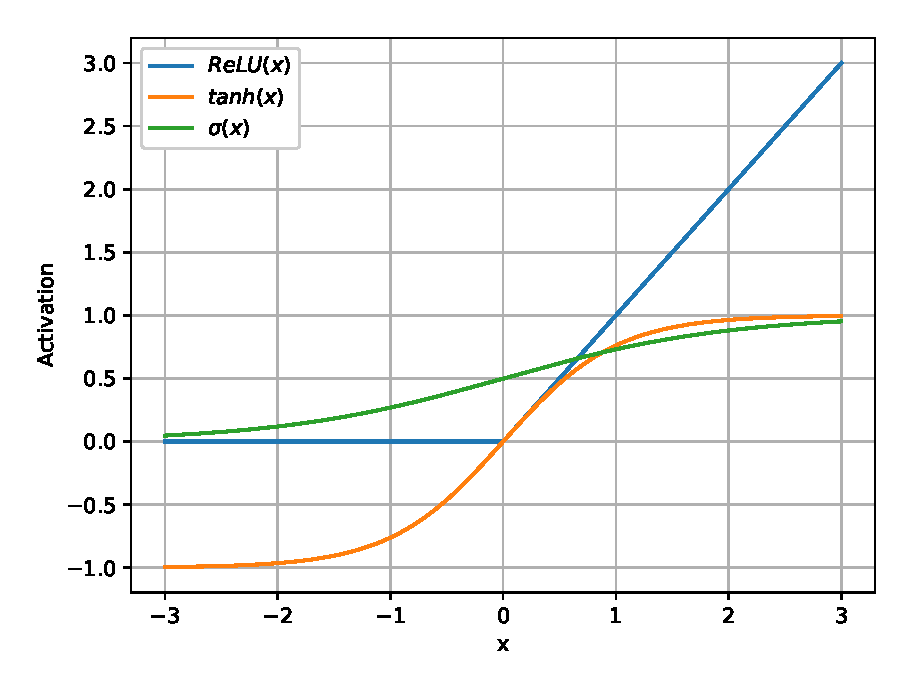
\includegraphics[width=0.6\textwidth]{chapters/NeuralNets/figures/Activations.pdf}
    \fonte{From the author(2021)}
    \label{fig:activations}
\end{figure}

This function can be useful to convert a single output to a probability value or to normalize a set of outputs. However, the fact that the outputs are always positive raises some problems, \textcite{efficientBackprop2012} showed that in these situations the backpropagation algorithm must update all the network parameters in the same direction, this means that the parameters are not free to wander the parameter space in the best direction.

Most of the time the network will benefit more by adding to some parameters while subtracting from others, the restriction to always update in the same direction makes learning more difficult and can greatly reduce the speed of convergence. \textcite{efficientBackprop2012} also argue that any deviation in the average of the outputs will bias the update direction, so it is better to have activations that are zero centered.

Knowing this problem, it only makes sense to consider sigmoid activations in the output layer, since for most cases it is better to use a zero centered alternative like the \gls{tanh} in the hidden layers.

\subsubsection{Hyperbolic Tangent}
The hyperbolic tangent function, as seen in \autoref{eq:tanh}, is a zero centered, scaled, and shifted version of the sigmoid function.
\begin{equation} \label{eq:tanh}
    \tanh(x) = \frac{e^x - e^{-x}}{e^x + e^{-x}} = 2\sigma(2x) - 1
\end{equation}

This function is almost always better than sigmoid since it has the same shape and properties without having the disadvantage of not being zero centered. It can be used in any layer, including the output. The times were a sigmoid would be preferred are when it is desired that the output be bounded to $(0,1)$, as is the case for a probability value.

\subsubsection{Rectified Linear Unit} \label{subsub:relu}
\glsreset{ReLU}
Both the sigmoid and hyperbolic tangent functions have two characteristics that can raise some problems when training a machine learning model. The first one is that they can only produce very close approximations of the number zero, but not the exact value \textbf{--} the only exception would be when the input of the \gls{tanh} function is also exactly zero, but this is very unlikely to happen and would only work for very specific inputs.

The lack of a true zero can be undesirable when the goal of the network is to build a sparse representation of the data, that is, a representation that only depends on a small number of inputs that strongly correlate to the output. This is in contrast with a model that depends on many inputs, but most of them have very little impact on the output.

The sparsity argument not only has some biological support, but has been shown to also positively influence the quality of a model \cite{relu2011}. Promoting sparsity is found in many other areas of science (e.g. statistical modeling, image compression) and it is very useful for producing simpler representations of the data \cite{dataDrivenScience2019}.

The other problem present in the sigmoid and \gls{tanh} functions is that they saturate for high absolute values of the input. Most of the variation in these functions occur close to zero, but for larger values there is barely any difference between outputs. For example, the difference between the \gls{tanh} activation between inputs $1$ and $2$ is around $0.2$, while the difference from $2$ to $100$ is just $0.036$. One other way to say this is that the derivatives of these functions are very close to zero for inputs far from the origin (see \autoref{fig:derivatives}), this can give rise to the vanishing gradients problem and make learning extremely slow (see \autoref{sub:vanishing_gradients}).
%
\begin{figure}[hbt]
    \centering
    \caption{Derivative of sigmoid, tanh and ReLU activation functions}
    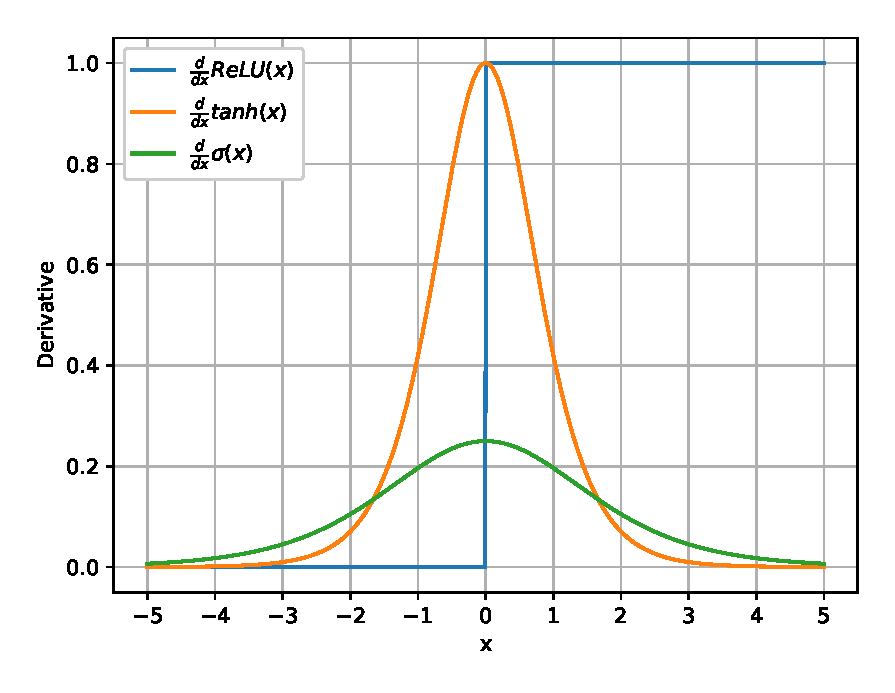
\includegraphics[width=0.6\textwidth]{chapters/NeuralNets/figures/Derivatives.pdf}
    \fonte{From the author(2021)}
    \label{fig:derivatives}
\end{figure}

The \gls{ReLU} activation function is an alternative that addresses both of the mentioned problems with sigmoid and \gls{tanh}. It is constructed from combining different linear regions (called a piecewise linear function), this allows for the activation to inherit many desirable properties of linear transformations while still retaining nonlinearity and being able to build complex relations \cite{deepLearningBook2016}.

The \gls{ReLU} function is simply composed of a constant zero for all negative inputs and the identity function for everything else, this means that for an input $x$ the activation is calculated as shown in \autoref{eq:relu}.
\begin{equation} \label{eq:relu}
    \ReLU(x) = \max(0, x)
\end{equation}

This definition allows for \gls{ReLU} to produce exact zeros for any negative inputs, promoting sparsity in the model representations. The constant positive derivative (see \autoref{fig:derivatives}) also removes the problem of vanishing gradients, since the units never saturate. Another big advantage of \gls{ReLU} is that it is extremely easy to compute, a simple \texttt{if} statement is enough to get the result; compared with the need to calculate exponentials in the sigmoid and \gls{tanh} functions, \gls{ReLU} performance is much faster.

Since around 2010, with papers like \cite{relu2011} exploring the \gls{ReLU} activation, there were many popular methods that showed impressive results using this function (e.g. \cite{alexnet2012} and \cite{inceptionV3_2015}). At the current time \gls{ReLU} is the standard recommended activation function to be used in most problems \cite{deepLearningBook2016}.

There are however some downsides to this activation. First there is the sharp change in the function behavior at the value $0$, making it's derivative undefined at that point, this however does not seem to be a problem in practice \cite{relu2011}. \gls{ReLU} also loses the desirable zero centered property that made \gls{tanh} a good substitute for the sigmoid, the argument from \textcite{efficientBackprop2012} holds for all activations, this means that all the network updates for units that use \gls{ReLU} must be made in the same direction, making learning more difficult.

Lastly, for a unit to be able to learn it is necessary that it outputs a value in the range where the activation function has a non-zero derivative for at least one example in the training data. But it is possible that for all the training data in a given problem, there exists some units using \gls{ReLU} activations that will always output zero, this makes learning impossible in these units and effectively freezes them on their state forever.

There are many other alternatives proposed to address these problems, some relevant examples are Maxout, LeakyReLU, ELU, GELU and PReLU, these have found some success in big machine learning problems\footnote{
    GELU is used in natural language processing models like GPT-3 \cite{gpt3_2020}
} and the benchmark by \cite{CaffeNetBench2017} showed good results for some of these alternatives \textbf{--} although \gls{ReLU} also fared well in those tests.

Between these alternatives, LeakyReLU is specially relevant for \acp{GAN}, being an important piece of the \glsunset{DCGAN}\gls{DCGAN} variant that is the base of many \gls{GAN} architectures. It consists of a simple change from ReLU that just guarantees that the units will always have at least some positive derivative. This activation is calculated as shown in \autoref{eq:leaky_relu}, where $\alpha$ is a hyperparameter that must be a small value (usually $0.3$).
\begin{equation} \label{eq:leaky_relu}
    \LeakyReLU(x) = \max(\alpha x, x)
\end{equation}

\subsubsection{Softmax}
In classification problems it is very common to have the output layer encode the input class has a $n$ dimensional, one-hot encoded vector, where $n$ is the number of classes. Since in one-hot encoding each element corresponds to the probability of the input belonging to the corresponding class (all zeros and a single $1$ for the correct class), it is desirable for the output of a classification model to also be a probability distribution. Besides the fact that it aligns with the encoding representation, it also gives a meaningful representation for the output of the network, by observing the output probabilities it is possible to have an idea of how confident the network is in the results\footnote{
    Since the values in a probability distribution should always add to $100\%$ this may not always give good representations, this is the case for adversarial examples that can fool the network to misclassify images with a high degree of confidence \cite{adversarialExamples2013}.
}.

The softmax activation function offers a way to map all the units weighted inputs to a probability distribution. One difference when compared to the other activation functions is that the softmax does not take a single number as input, instead it uses all values in the layer for calculating the unit activation. This makes sense since the probabilities are dependent on the proportions of each unit weighted input. \autoref{eq:softmax} shows how the activation for the unit $i$ is calculated based on the layer weighted inputs $(z_0 \dots z_n)$, the layer superscripts were omitted for clarity.
\begin{equation} \label{eq:softmax}
    a_i = \frac{e^{z_i}}{ \sum\limits_{k=0}^{n}{e^{z_k}} }
\end{equation}
